% ======================================================== %
% Przeczytaj plik amuthesis-doc.pdf, aby poznać opcje      %
% klasy `amuthesis`                                        %
% ======================================================== %
\documentclass[oneside,polski,logo]{amuthesis}

% Zdefiniuj kodowanie pliku źródłowego (domyślnie utf8)
\usepackage[utf8]{inputenc}
\usepackage[nottoc,notlot,notlof]{tocbibind}

% ======================================================== %
% Dane autora i pracy                                      %
% ======================================================== %

% --- Autor pracy
\author{Kamil Tyrek, Mateusz Hypś, Jakub Kozubal}
% --- Numer albumu
\album{434797, 434699, 434726}
% --- Tytuł pracy (w języku polskim i angielskim)
\titlePL{Projekt i implementacja gry „The Lore: Story of the fallen warrior”}
\titleEN{Project and implementation of game „The Lore: Story of the fallen warrior”}
% --- Typ pracy (inżynierska, licencjacka, magisterska)
\type{inżynierska}
\graphicspath{ {./images} }
% --- Wydział (wykaz skrótów):
% --- --- WA    --- Wydział Anglistyki
% --- --- WB    --- Wydział Biologii
% --- --- WCh   --- Wydział Chemii
% --- --- WFPiK --- Wydział Filologii Polskiej i Klasycznej
% --- --- WF    --- Wydział Fizyki
% --- --- WH    --- Wydział Historyczny
% --- --- WMiI  --- Wydział Matematyki i Informatyki
% --- --- WNGiG --- Wydział Nauk Geograficznych i Geologicznych
% --- --- WNPiD --- Wydział Nauk Politycznych i Dziennikarstwa
% --- --- WNS   --- Wydział Nauk Społecznych
% --- --- WN    --- Wydział Neofilologii
% --- --- WPAK  --- Wydział Pedagogiczno-Artystyczny w Kaliszu
% --- --- WPiA  --- Wydział Prawa i Administracji
% --- --- WSE   --- Wydział Studiów Edukacyjnych
% --- --- WT    --- Wydział Teologiczny
% --- --- IKE   --- Instytut Kultury Europejskiej w Gnieźnie
\faculty{WMiI}
% --- Kierunek (w mianowniku)
\field{informatyka}
% --- Specjalność (w formie mianownikowej)
% --- (ustaw puste, jeśli bez specjalności)
% --- Promotor (w dopełniaczu)
\supervisor{dr Bartłomieja Przybylskiego}
% --- Data złożenia pracy (Miasto, miesiąc rok)
\date{Poznań, styczeń 2021}

% --- Płeć autora (M/K)
\stsex{M}
% --- Zgoda na udostępnienie pracy w czytelni (TAK/NIE)
\stread{TAK}
% --- Zgoda na udostępnienie pracy w zakresie ochrony (TAK/NIE)
\stprotect{TAK}
% --- Data podpisania oświadczenia (Miasto, data)
\stdate{Poznań, \today{} r.}

% ======================================================== %
% Dodatkowe pakiety wykorzystywane w pracy                 %
% ======================================================== %

\usepackage{lipsum}

% ======================================================== %
% Zasadnicza część dokumentu                               %
% ======================================================== %

\begin{document}

% Strona tytułowa
\maketitle
% Oświadczenie
\makestatement
% Spis treści
\tableofcontents
\addcontentsline{toc}{chapter}{Bibliography}


% ======================================================== %
% Właściwa część pracy                                     %
% ======================================================== %

\chapter{Wstęp}
\section{Cel i założenia projektu}
Celem projektu jest stworzenie gry platformowej, zawierającej elementy zręcznościowe oraz łamigłówki. Głównym założeniem projektu jest gra, która zaciekawi swoją fabułą oraz trudnością. Wstępnie prosty zamysł samouczka, w większości gier jest raczej elementem wprowadzającym do rozgrywki, która powinna robić się trudniejsza w im dalszym etapie rozgrywki się znajdujemy, w przypadku naszej gry jest odwrócony. Samouczek poza wprowadzaniu poszczególnych elementów rozgrywki, którymi jest między innymi przedstawienie sterowania oraz funkcjonalności i wstępnych mechanik jest również wymagający, od gracza zależy jakie umiejętności w trakcie rozgrywki będzie rozwijać, aby przejście kolejnych poziomów było łatwiejsze (z perspektywy gracza). Dużą wagę w projekcie przywiązujemy do mini-gier, które występują w trakcie przechodzenia poszczególnych poziomów. Występują dwa rodzaje mini-gier: opcjonalne (te które przejść możemy w celu sprawdzenia siebie oraz zdobycia punktów doświadczenia) oraz wymagane, które trzeba przejść, aby znaleźć się w dalszym etapie gry. Użytkownik posiada do dyspozycji punkty doświadczenia, drzewko umiejętności oraz ekwipunek. Punkty doświadczenia możemy wydawać bezpośrednio w drzewku umiejętności, w którym zadaniem gracza jest wybranie odpowiednich umiejętności zależnie od tego jaką strategię rozgrywki chce przyjąć. Warto pamiętać jednak, że im głębiej będziemy rozwijać daną gałęź tym umiejętności będą bardziej pomocne co sprawia, że gracz musi zastanowić się dobrze nad decyzjami dotyczącymi rozwijania konkretnych umiejętności w drzewku. Ekwipunek służy do zdobywania przedmiotów potrzebnych w trakcie rozgrywki m.in. do otwierania drzwi czy rozpoczęcia opcjonalnej mini-gry. W projekcie są wykorzystane 2 style tworzenia poziomów: ortographic i perspective. Wszystkie animacje w projekcie są tworzone z użyciem technologii inverse kinematics co pozwala na stałe dodawanie nowych animacji i poprawianie już istniejących.
\section{Organizacja pracy}
Charakter projektu sprawił, iż nie można w naszym zespole jasno podzielić typów zadań, które realizujemy w ramach projektu. Wynikiem tego jest to, iż nowe funkcjonalności są realizowane zazwyczaj przez jedną osobę od początku do końca, nie ma podziału, podobnego jak w przypadku aplikacji z frontendem i backendem.


Jako metodykę pracy przyjęto Scrum. Głównymi powodami tej decyzji jest doświadczenie części zespołu w tej metodyce oraz przejrzystość i rozsądne zarządzanie pracą. Nie rozważano innych metodyk pracy. Przy zarządzaniu pracą wspomaga nas serwis JIRA, który pozwala zarządzać regularne sprinty – w pierwszym semestrze dwutygodniowe, w drugim semestrze tygodniowe. 


Kod źródłowy zarządzany jest poprzez GitHub. Dla przejrzystości pracy, każdy commit na GitHub oznaczany jest id zadania na Jirze, dzięki czemu wchodząc w zadanie widzimy commit powiązany z jego rozwiązaniem. W momencie rozpoczęcia zadania deweloper, jeśli następuje potrzeba, tworzy podzadania do zadań na Jirze. Dotyczy to większych zadań, których wykonanie polega na tworzeniu większej ilości funkcjonalności. Dzięki temu realizując nowe zadania, o podobnej budowie, można sugerować się podobnym sposobem działania zadania. Po każdym commicie programista wyznacza ile czasu poświęcił na zadanie, poprzez wbudowaną w Jirze funkcjonalność “Log Work”. Gdy zadanie zostanie zakończone, programista oznacza je statusem “DONE”.  


Z racji wybranej metodyki, dokonano również przydzielenia odpowiednich ról członkom zespołu. Podział ról wygląda następująco:

\begin{itemize}
	\item Kamil Tyrek - Development Team, Scrum Master
	\item Jakub Kozubal -Development Team, Product Owner
	\item Mateusz Hypś - Development Team
\end{itemize}

\section{Podział prac}
\subsection{Kamil Tyrek - tworzenie elementów logicznych i ich algorytmika}
W tym rozdziale zostaną przedstawione sposoby tworzenia elementów logicznych. Część z przedstawionych łamigłówek została użyta w projekcie końcowym. Przykładem są tutaj przesuwane puzzle - rozgrywka polegająca na przesunięciu elementu, celem ułożenia poprawnego obrazka. Algorytmika stojąca za losowaniem kolejności elementów nie jest trywialna, ponieważ źle wylosowana kolejność puzzli powoduje, iż mogą być niemożliwe do ułożenia.

Zostanie przedstawiona też logika mini-gry z ustawieniem odpowiednich ruch, celem połączenia dwóch końców rur. Podobnie jak w poprzednim przykładzie, do rozwiązania tej zagadki potrzebna jest odpowiednia liczba rur danego typu - pionowe, poziome, skrętne. 

Następnym przykładem będzie logika stojąca za rozgrywką, która nie jest dostępna w końcowym projekcje, a chodzi tutaj o generowanie labiryntu. Nietrywialnym problemem jest wygenerowanie takiej planszy, aby możliwe było przejście z punktu A do punktu B. W tym rozdziale postaramy się przedstawić rozwiązanie tego problemu, przy użyciu odpowiednich algorytmów.

\subsection{Mateusz Hypś - Zarządzanie projektem gry komputerowej z wykorzystaniem Agile}
W rozdziale zostanie opisany proces zarządzania projektem z wykorzystaniem metodyki zwinnej. Omówione i porównane zostaną podejścia Agile i Agile Game Development oraz zastosowania tych metodyk, w porównaniu z innymi stosowanymi w praktyce. Przedstawione zostaną najważniejszych idee stojące za metodykami Agile m.in. framework SCRUM. Następnie omówione zostanie zastosowanie tych metodyk w projekcie “The Lore”, z uwzględnieniem problemów w trakcie realizacji tego projektu. 
\subsection{Jakub Kozubal - Fizyka postaci}
W tym rozdziale zostaną przedstawione sposoby tworzenia poruszania się postaci. Zaznaczone zostaną główne różnice między fizyką rzeczywistą, a tą stosowaną w grach jak i przedstawienie wielu sposobów rozwiązania tej samej funkcjonalności. Ponadto przedstawiony zostanie proces tworzenia postaci. Do tego pojawi się też opisanie problemów takich jak sterowanie postaci w powietrzu oraz oddziaływanie sił z otoczenia (m.in. poruszające się platformy). Zostanie także przedstawione i przeanalizowane działanie każdej umiejętności występującej w drzewku odpowiedzialnej za poruszanie się.

\section{Użyta technologia - Unity}
 W naszym projekcie postanowiliśmy wybrać UNITY jako środowisko do stworzenia naszej gry. Wynikało to z możliwości jakie oferuje oraz z jakości i czytelności, stworzonej przez twórców, oficjalnej dokumentacji. Pozwala nam na tworzenie gier dwuwymiarowych czy trójwymiarowych oraz interaktywnych materiałów, na przykład animacje czy wizualizacje. W razie problemów możemy również wykorzystywać oficjalne forum na którym rzesza użytkowników dzieli się swoimi wskazówkami a także oficjalny sklep – Asset Store, w którym możemy wykupić materiały potrzebne do naszej gry. UNITY działa na każdym systemie operacyjnym, tj. Windows, macOS oraz Linux. Gwarantuje nam również możliwość stworzenia aplikacji nie tylko na komputery osobiste, ale także przeglądarki internetowe, konsole gier wideo oraz urządzenia mobilne. Dzięki aktualizacji silnika do wersji 5.1.1 ta lista wzrasta do 22 platform sprzętowych, w tym gogle wirtualnej rzeczywistości takie jak Oculus Rift.
W przeszłości można było tworzyć aplikacje w trzech językach:
\begin{itemize}
	\item UnityScript (swego rodzaju pochodna JavaScript’u)
	\item C\#
	\item Boo
\end{itemize}
Jednak wraz z piątą wersją silnika (wydaną w roku 2015) możliwość pisania w języku Boo została usunięta, pozostała tylko wsteczna kompatybilność w postaci możliwości kompilacji skryptów przez środowisko MonoDevelop. Podobny los dotknął UnityScript, którego wsparcie zakończyło się na wersji 2018.2 (najnowsza wersja stabilna to 2019.3.4). Z tych względów nasz wybór musiał paść na język C\#, w którym zostały napisane wszystkie nasze skrypty. Jako jedyny jest wciąż wspierany przez autorów, co zaowocowało drastycznym wzrostem popularności wśród użytkowników.

\chapter{Zarządzanie projektem gry komputerowej z wykorzystaniem Agile}
\section{Czym jest projekt?}
Aby odpowiednio przyswoić temat zarządzenia projektem, należy zacząć od zrozumienia paru terminów  które są nieodłączną jego częścią. 
Projekt jest to termin z pozoru banalny, w końcu spotykamy się z nim wielokrotnie, jednak wytłumaczenie go może sprawiać problemy. Jedną z najlepszych oraz najbardziej wyczerpujących definicji na jaką można trafić jest ta stworzona przez Roberta K. Wysockiego oraz Rudd’a McGary'ego. Są to Amerykańscy specjaliści w temacie zarządzania projektami. W ich książce pod tytułem „Efektywne zarządzanie projektami” definiują projekt jako: „sekwencję niepowtarzalnych, złożonych i związanych ze sobą zadań, mających wspólny cel, przeznaczonych do wykonania w określonym terminie bez przekraczania ustalonego budżetu, zgodnie z założonymi wymaganiami”. \cite{projekt}

Pomimo faktu iż powyższa definicja jest najprawdopodobniej znacznie bardziej złożona od takiej którą słyszymy na co dzień to jest ona bardzo cenna, ponieważ przedstawia najważniejsze cechy każdego projektu.

Składa się z czterech podstawowych elementów, którymi menedżer projektu musi zarządzać symultanicznie. Trzeba pamiętać, że są one ze sobą powiązane. Do wspomnianych elementów należą: 
\begin{itemize}
	\item Zakres
	\item Zasoby
	\item Czas
	\item Pieniądze
\end{itemize}

\subsection {Zakres}
Zdecydowanie najważniejszy z całej czwórki. Jest on definicją co tak naprawdę projekt ma osiągnąć i co ma w nim zostać zrealizowane. Obrazuje rozmiar projektu, jego cele a także wymagania. Zakres jest nie tylko najważniejszym, ale również najbardziej złożonym. Jakakolwiek zmiana musi zostać odwzorowana w pozostałych trzech elementach. Jest to jeden z powodów dla którego się mówi o współzależności między tą czwórką. Aby to lepiej zrozumieć, można sobie wyobrazić aplikacje, która ma posiadać cztery główne funkcjonalności, zbudowana przez dwa zespoły z budżetem 40 tysięcy złotych. Jeśli zakres projektu się zmieni do przykładowo sześciu funkcjonalności, zadaniem menedżera projektu jest dostosowanie zasobów ludzkich, czasu oraz budżetu w taki sposób aby cel ten został zrealizowany.

\subsection {Zasoby}
Zasoby dzielą się na trzy kategorie:
\begin{itemize}
	\item Zasoby ludzkie
	\item Wyposażenie
	\item Materiały
\end{itemize}
\subsubsection {Zasoby ludzkie}

Menadżer projektu musi upewnić się że pracownicy posiadają odpowiednie umiejętności i narzędzia aby ukończyć dane im zadanie. Musi w pełni monitorować czy ma wystarczającą ilość zasobów ludzkich do konkretnego projektu tak aby go ukończyli w ustalonym czasie. Jego zadaniem jest również dopilnowanie aby każda osoba przypisana do zadania doskonale wiedziała i rozumiała co ma zrobić oraz znała wyznaczone terminy. W większych firmach wygląda to inaczej. Pracownicy są podzieleni na grupy którymi zarządza team leader, jest on odpowiedzialny za większość obowiązków które zostały wymienione powyżej. Wynika to z faktu iż menedżer projektu nie jest w stanie zarządzać tak dużym zbiorowiskiem ludzi. Dużym atutem jest również to że team leader najlepiej zna swój zespół, ich umiejętności, możliwości, a także czas którym dysponują. Jest to również duże ułatwienie dla menedżera projektów ponieważ nie musi komunikować się ani nadzorować wszystkich, wystarczy kontakt z team leaderem konkretnych zespołów. 

\subsubsection {Wyposażenie i materiały}
Czasami dochodzi do sytuacji, w której project manager jest odpowiedzialny za pozyskiwanie materiałów i wyposażenie którymi musi zarządzać w taki sposób aby zespół wykonywał swoją prace w najefektywniejszy sposób. Nie jest to często spotykane zjawisko, w szczególności w dużych firmach w których podzial obowiązków jest mocniej rozdzielony po wielu pracownikach.

\subsection {Czas}
Podobnie jak w przypadku zasobów, czas jest dzielony na trzy grupy
\begin{itemize}
	\item Podział na zadania
	\item Harmonogram
	\item Ścieżka krytyczna (ang. Critical path)
\end{itemize}

\subsubsection {Podział na zadania}
Podział na zadania jest pierwszym z trzech kroków do pomyślnego zarządzania czasem. Zadania muszą być tworzone w przemyślany sposób, dobrze przeanalizowane, a także odpowiednio wytłumaczone, tak aby pracownik, który się go podejmie, wszystko zrozumiał za pierwszym razem. Niespełnienie przynajmniej jednego z wyżej wymienionych warunków tworzenia zadań negatywnie wpływa na ich wykonanie. W wielu przypadkach łączy się to z opóźnieniami w realizacji projektu.

\subsubsection {Harmonogram}
Po pomyślnym stworzeniu zadań przechodzi się do zaplanowania harmonogramu. Tworzy się go poprzez listowanie w odpowiedniej kolejności wszystkich zadań, które muszą zostać wykonane. Niektóre z nich można wykonywać sekwencyjnie, inne z nich mogą nakładać się na siebie, a jeszcze inne mogą zostać wykonane jednocześnie. Kluczem do sukcesu jest ich zrozumienie i poprawne grupowanie. Następnym ważnym czynnikiem jest zrozumienie zależności między nimi, ponieważ niektóre z zadań muszą zostać wykonane w pierwszej kolejności. Ostatnim krokiem tworzenia harmonogramy jest estymacja czasu potrzebnego do ich wykonania, a także przypisanie im odpowiednich zasobów. 

\subsubsection {Ścieżka krytyczna (ang. Critical path)}
Niektóre zadania mają elastyczny termin rozpoczęcia oraz ich zakończenia. Jednak istnieją również takie które tej elastyczności nie mają. Linia przechodząca przez zbiór takich zadań nazywana jest ścieżką krytyczną i wykorzystywana jest do monitorowania w jakim tempie zostają wykonywane zadania w projekcie. W zależności od podziału zadań, istnieje możliwość występowania wielu ścieżek krytycznych. Wszystkie zadania które znajdują się na ich drodze muszą zostać wykonane w terminie, w przeciwnym razie występuje bardzo wysokie prawdopodobieństwo że projekt nie zostanie ukończony na czas.

\subsection {Pieniądze}
Dla najefektywniejszego zarządzania kosztami projektu uwzględnia się jego:

\begin{itemize}
	\item Koszty
	\item Wydatki związane z losowymi zdarzeniami
	\item Zyski
\end{itemize}

\subsubsection {Koszty}
Każde zadanie ma określony koszt potrzebny do jego do wykonania, najczęściej bazuje na wydatkach związanych z potrzebnymi zasobami. Każdy z tych wydatków jest estymowany i uwzględniany podczas przygotowania budżetu dla projektu.

\subsubsection {Wydatki związane z losowymi zdarzeniami}
Podobnie jak w estymacji czasu potrzebnego do wykonania konkretnych zadań, tak samo przy przygotowywaniu budżetu należy uwzględnić pewien bufor. Zostanie on wykorzystany na wypadek losowych zdarzeń, które mogą się w nieoczekiwanym momencie wydarzyć. Najprostszym przykładem w firmie informatycznej może być problem techniczny związany ze sprzętem np. zepsuty komputer.

\subsubsection {Zyski}
Zyski są to pieniądze, które firma planuje zarobić na wykonanym projekcie, bądź po każdym zakończonym zadaniu. Oczywiście aby projekt został uznany za opłacalny dla biznesu, budżet, który zawiera odpowiednio oszacowane koszty nie może przekraczać pewnego procentu planowanych zysków. Zadaniem menedżera projektu jest oczywiście zminimalizowanie jak najbardziej kosztów produkcji i jak największe zmaksymalizowanie zysku, które firma zarobi po wykonanym projekcie.


\section {Czym jest zarządzanie projektem}
Po dokładnym zaznajomieniu się czym jest projekt, zrozumienie na czym polega zarządzanie projektem staje się trywialne. Jest to proces, którego celem jest ukończenie projektu zgodnie z określonymi wymaganiami (najczęściej czasowymi i budżetowymi), do jego realizacji stosuje się wiedzę, narzędzia, umiejętności, oraz odpowiednie techniki. 
\begin{figure}[h]
	\centering
	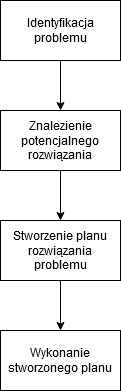
\includegraphics[width=4cm]{images/hyps/diagram-zarzadzania-projektem.png}
	\caption{Uproszczony proces realizacji projektu}
\end{figure}

Powyższy diagram obrazuje proces realizacji projektu w bardzo uproszczonym formacie, ponieważ każdy etap kryje za sobą wiele procesów które trzeba dodatkowo wykonać.
\subsubsection {Project manager}


\subsection{Cykl życia projektu informatycznego}
\subsection{Metody pomocne w zarządzaniu projektami informatycznymi}
\subsection{Ryzyko oraz powody niepowodzeń  projektów informatycznych}

\section{Zarządzanie projektem gry komputerowej - The Lore}
\subsection{Proces planowania projektu}
\subsection{Wykorzystane systemy i metody projektowe}
\subsection{Rola i wpływ kierownika projektu} 
\subsection{Cykl życia projektu The Lore}

\chapter{Zagadki logiczne}
\section{Wprowadzenie do zagadek logicznych}
\subsection{Omówienie zagadnienia}
Zagadką logiczną określamy zadanie, którego celem jest odnalezienie odpowiedzi na pytanie, logiczne dojście do rozwiązania problemu czy też czasami abstrakcyjne myślenie. Możemy wyróżnić różne rodzaje zagadek, między innymi graficzne, czego przykładem jest znany, często używany w szkołach podstawowych rebus. Główną ideą takiej rozgrywki jest rozwój swoich intelektualnych możliwości przy dobrej zabawie. \cite{zagadka_logiczna}
\subsection{Przykłady logicznych zagadek w prawdziwym świecie}
\subsubsection{Rebus}
Przywołanym już przykładem zagadki może być rebus. To prosta rozgrywka, polegająca na odgadnięciu hasła na podstawie przytoczonego obrazka. Często treści w rebusach mogą być niejednoznaczne, co sprawia, iż nie są one trywialne i wymagają wielu kombinacji haseł, związanych z danym obrazkiem. \cite{rebus}
\begin{figure}[h]
	\centering
	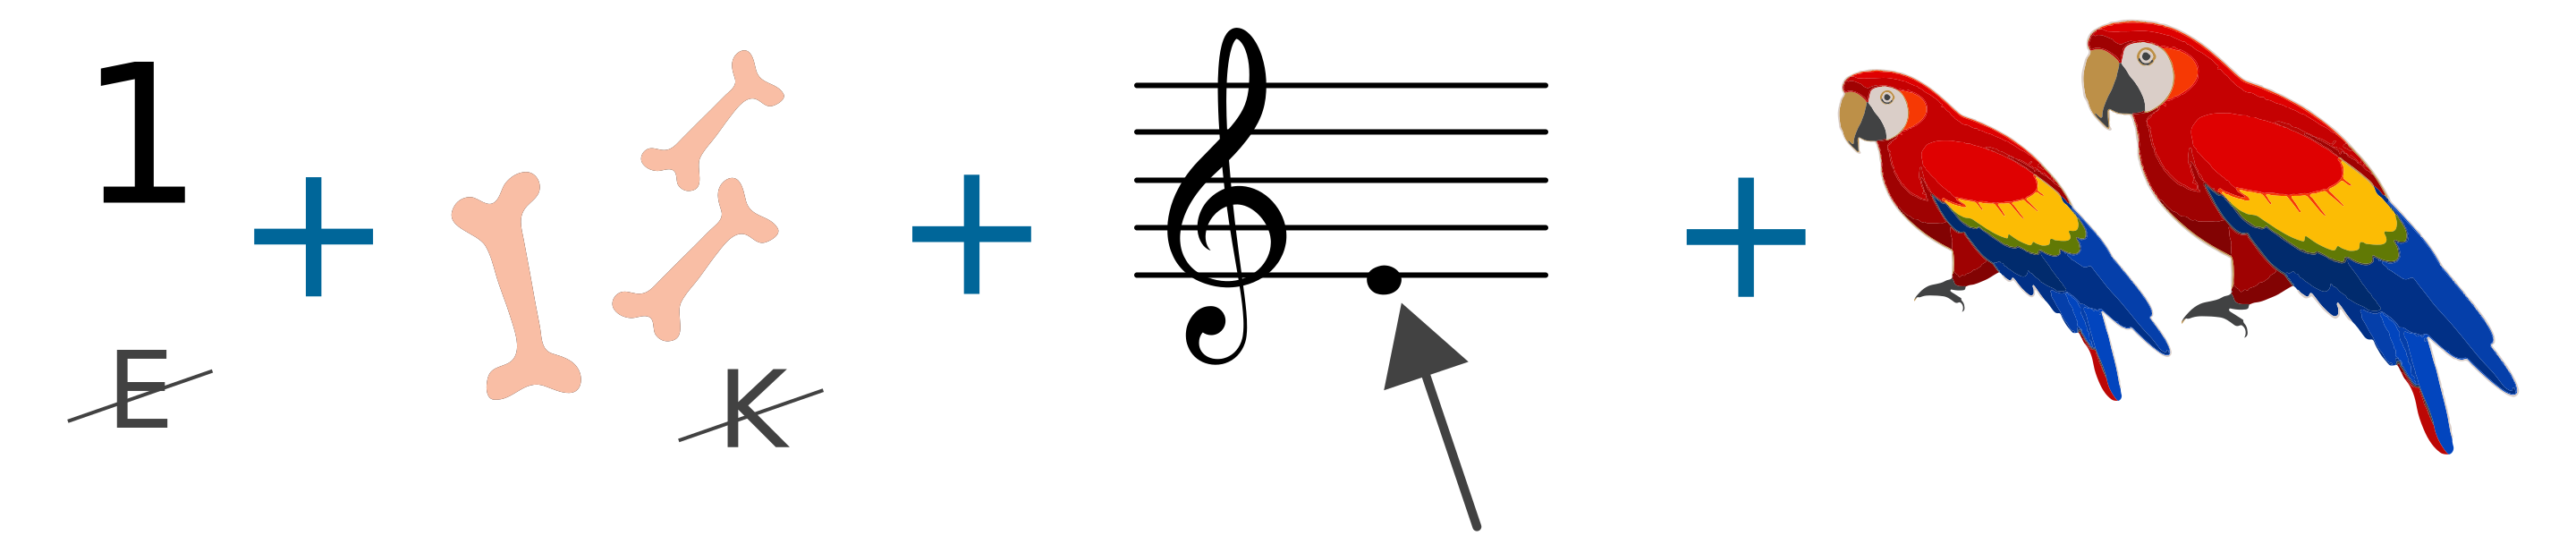
\includegraphics[width=8cm]{images/tyrek/rebus.png}
	\caption{Źródło: Zespół autorski Politechniki Łódzkiej, licencja: CC BY 3.0}
\end{figure}

\subsubsection{Piętnastka - przesuwane puzzle}
Kolejnym przykładem może być też piętnastka, która w grze The Lore została zaimplementowana jako przesuwane puzzle rozmiarów 3 na 3. Temat szerzej poruszony będzie w dalszej części pracy, gdzie oprócz założeń związanych z rozwiązaniem zagadki, przedstawiona będzie logika idąca za zrealizowaniem tej zagadki w grze opartej na silniku Unity. 
\begin{figure}[h]
	\centering
	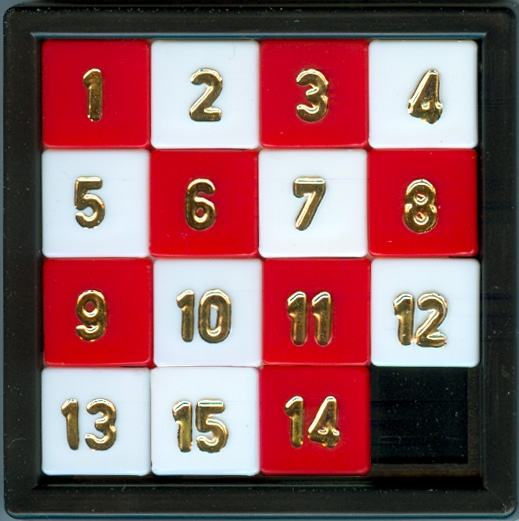
\includegraphics[width=5cm]{images/tyrek/przesuwane-puzzle.jpg}
	\caption{Źródło: Wikipedia, Sliding Puzzle, Micha L. Rieser - Public Domain}
\end{figure}

\subsubsection{Puzzle}
Jedną z najpopularniejszych zagadek logicznych, z którą styczność miał zapewne każdy z nas, są puzzle. Jest to gra, w czasie której rozwiązajemy problem polegający na ułożeniu z dostępnych elementów logicznego obrazka, który zazwyczaj jest dołączony do gry - w postaci fotografii czy też po prostu znajduje na pudełku.   
 
Słowo puzzle pochodzi z XVI wieku, które oznaczało "stan zagubienia". Sama gra ma swoje początki w wieku XVIII, gdy John Spilsbury, grawer i kartograf umieścił mapę na drewnie, następnie przepiłował ją wokół konturów każdego kraju znajdującego się na mapanie. To co powstało postanowił użyć do nauki geografii - ułożenie logicznej mapy uczyło jak wygląda mapa danego regionu. Taka pomoc dydaktyczna zdobyła szybko popularność, wszak była to nauka przez zabawę, używano ją dość często, nawet jeszcze w wieku XIX.  

Trudność puzzli zależy zazwyczaj od kształtu elementów i ich ilości. Jeżeli chodzi o kształt, puzzle często mają specyficzny kształt, przez co nie każdy element pasuje do innego, co pozwala nam odrzucić możliwości połączenia różnych par. Ilość elementów zwiększa ilość możliwych oraz logicznych kombinacji danych elementów, przez co zwiększa się czas realizacji zadania. Największa układanka została wykonana przez firmę Educa, posiadała ona aż 42 000 elementów i przedstawia dość bajeczny krajobraz, na którym znajdują się najpopularniejsze budynki z całego świata - Big Ben, Wieża Eiffela czy Krzywą Wieżę w Pizie. Ułożenie tej układanki możemy liczyć w setkach godzin. \cite{puzzle}

\begin{figure}[h]
	\centering
	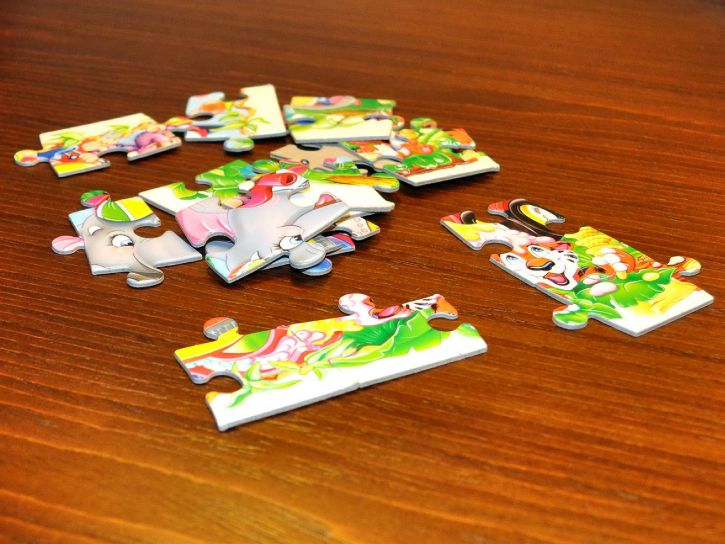
\includegraphics[width=5cm]{images/tyrek/puzzle.jpg}
	\caption{Źródło: Pixnio, Przykład puzzli - Public Domain}
\end{figure}

\subsection{Wdrożenie zagadek do gry opartej na silniku Unity}
\subsubsection{Scena w Unity}
W Unity możemy podzielić naszą grę na sceny. Scena to obiekt zawierający nasze menu, czy dane środowisko gry (na przykład poziom gry). Dobrą praktyką jest, aby każdy level gry był osobą sceną, co skróci czas jego ładowania. W scenie możemy umieścić swoje obiekty, skrypty czy grafiki. \cite{scena}
\subsection{Obiekt - GameObject}
Obiekt, zwany w Unity GameObject, to klasa podstawowa dla wszystkich podmiotów w scenach Unity. Do każdego obiektu możemy przypinać kolejne obiekty, tworząc hierarchiczność, która może się przydać w odpowiedniej realizacji projektu. \cite{gameobject}
\begin{figure} % TODO - obrazek w złym miejscu
	\centering
	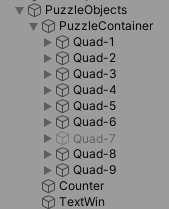
\includegraphics[width=4cm]{images/tyrek/hierarchia.png}
	\caption{Hierarchia obiektów. Przykład z projektu The Lore}
\end{figure}
\subsection{Sposoby dodawania mini-gier}
W toku pracy nad projektem The Lore rozpatrywano dwa sposoby dodawania mini-gier do gry:
\begin{itemize}
	\item{Każda minigra jest w osobnej scenie}
	\begin{itemize}
		\item W przypadku rozbudowanych poziomów nie powiela szerokiej listy obiektów sceny
		\item Pozwala na mniejsze pobieranie zasobów w danej jednostce czasu - połączenie działającego poziomu z algorytymką mini-gry może bywać uciążliwe na słabszych komputerach.
	\end{itemize}
	\item{Każda minigra zawiera się w scenie poziomu gry}
		\begin{itemize}
		\item Unikamy dłuższego ładowania się poziomu gry. Po zakończeniu mini-gry w przypadku osobnej sceny, cały poziom musi załadować się od nowa.
	\end{itemize}
\end{itemize}
Po wewnętrznej dyskusji wybrano opcję wydzielenia do osobnej sceny. W toku testowania tego rozwiązania uznano, iż nie jest ono bardzo uciążliwe pod kątem czasu ładowania poziomu, zaś pozwala na zachowanie porządku w projekcie. Jak się okazało już w przypadku projektowania poziomu 1. gry, ta decyzja była właściwa. Z racji sporego rozbudowania tego obiektu i dużej liczby obiektów, dodanie mini-gier do tej sceny mogłoby spowodować chaos organizacyjny.
\section{Przesuwane puzzle}
\subsection{Omówienie zagadnienia i ogólne założenia}
Przesuwane puzzle to układanka, złożona zazwyczaj z kwadratowej liczby elementów, najczęściej jest to szesnaście pól. Pola są jednakowych rozmiarów i oznaczone są liczbami od 1 do (n-1), gdzie n to liczba dostępnych pól w układance. Jedno pole jest puste, pozwala to na przeniesienie sąsiednich elementów puzzli względem siebie. Rozgrywka kończy się, gdy ułożymy puzzle w odpowiedniej kolejności, według rosnącego porządku liczb lub powstania odpowiedniego obrazka. Trudno określić kto odpowiada za stworzenie zagadaki. Wiadomym jest, że w 1878 roku pochodzący ze Stanów Zjednoczonych Samuel Loyd wypromował układankę, jednak prawdopodobnie nie jest to jego pomysł. Dość popularną nazwą na rozgrywkę jest "piętnastka", określającą ilość dostępnych pól w najpopularniejszym ułożeniu - 4x4.  \cite{sliding_puzzle}

W grze The Lore gracze staną przez rozwiązaniem zagadki gdzie do dyspozycji mamy dziewięć pól. Podczas projektowania układanki w grze uznano, iż zagadka może być dość trudna, a korzyści płynące z rozwiązania jej będą nieadekwatne do poświęconego czasu, stąd ilość pól jest mniejsza niż w najpopularniejszej wersji rozgrywki.
\subsection{Algorytmika}
\subsubsection{Pojedynczy element puzzle - PuzzleBlock}

Każdy pojedynczy element puzzla jest zainicjalizowany jako obiekt, który określamy jako PuzzleBlock. Obiekt posiada koordynaty, które określają jego położenie w przestrzeni na układance.

\begin{figure}[h]
	\centering
	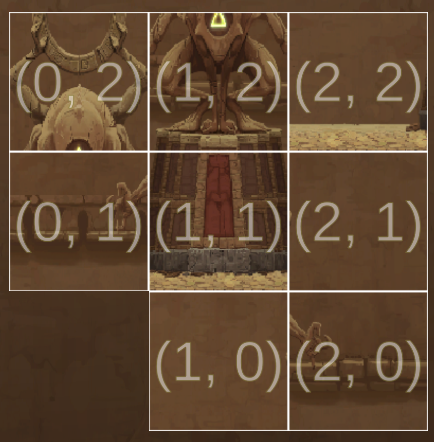
\includegraphics[width=6cm]{images/tyrek/coord_puzzle.png}
	\caption{Koordynaty każdego pola. Przykład z gry The Lore}
\end{figure}

Tak jak na załączonym przykładzie, wartość x rośnie w prawą stronę, zaś Y w górę, gdzie x dotyczy położenia w poziomie, a y w pionie. W założeniach przedstawiona została logika, która mówiła, iż element może zostać przemieszczony wtedy i tylko wtedy, gdy pole obok niego jest wolne, czyli nie posiada żadnego PuzzleBlock - elementu z liczbą lub obrazkiem. Dla lepszego efektu wizualnego, w grze The Lore element porusza się stopniowo, aby sprawiał wrażenie, iż porusza się realistycznie. Z racji, iż w Unity każda akcja wykonuje się podczas pokazywania kolejnej klatki, element porusza się w minimalnym stopniu przez sekundę. 

\subsubsection{Plansza - Puzzle. Losowanie kolejności puzzli}
Plansza rozgrywki posiada 8 elementów PuzzleBlock oraz jedno puste pole.  Algorytm powinien wylosować dla 8 pól ich położenie na planszy - tak jak w wyżej przedstawionym przykładzie. W tym celu na początku losujemy dla każdego bloku wartość od 0 do 8. W C\# możemy to zrobić przy użyciu funkcji  System.Random().Next(a, b). Przykładowo:
\begin{lstlisting}[
language={[Sharp]C},
rulecolor=\color{blue!80!black},
caption={Fragment klasy \texttt{Puzzle.cs}}
]
private int randomPosition()
{
    int pos = 0;
    do
    {
        pos = new System.Random().Next(0, 9);
    }
    while (isOnBoard[pos]);
    isOnBoard[pos] = true;
    return pos;
}
\end{lstlisting}

Gdzie isOnBoard[pos] jest tablicą, która weryfikuje, czy dane pole nie jest już zajęte. Jeśli jest, ponownie losujemy wartość dla PuzzleBlock. Oczywiście to nie koniec - z tej wartości musimy stworzyć położenie w postaci (x, y), gdzie x to położenie w poziomie, a y w pionie. W tym celu jedna z tych wartości będzie resztą dzielenia wylosowanej pozycji przez trzy (ilość pól w linii), a druga ilorazem całkowitym pozycji i liczby trzy. 
Kolejną ważną rzeczą będzie weryfikacja, czy obecne ułożenie puzzli jest wykonalne.

\subsubsection{Plansza - Puzzle. Weryfikacja kolejności puzzli}
Jak się okazuje niektóre ułożenia puzzli powodują, iż nie ma żadnego rozwiązania tego problemu. Z przypadkiem takiej sytuacji spotykaliśmy podczas pierwszych testów mini-gry puzzle. 
\begin{figure}[h]
	\centering
	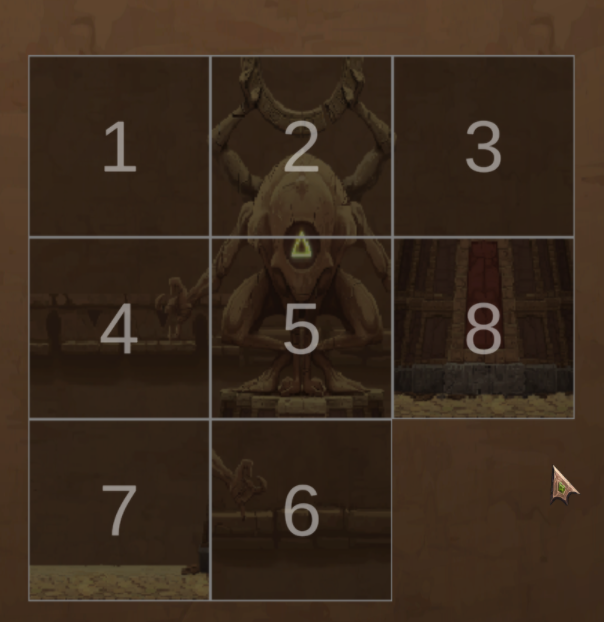
\includegraphics[width=5cm]{images/tyrek/puzzle_1.png}
	\caption{Puzzle bez rozwiązania. Przykład z gry The Lore}
\end{figure}

Jak się okazuje, występuje tutaj dość prosta zasada. Łamigłówka przesuwanych puzzli z 8 elementami jest rozwiązywalna wtedy i tylko wtedy, gdy liczba inwersji stanu początkowego jest parzysta. Czym jest zaś w tym przypadku liczba inwersji?

Inwersją nazwiemy parę liczb, której wartości są w odwrotnej kolejności, niż w zakładanym stanie końcowym. \cite{solvablePuzzle} Przyjmijmy taką sytuację:

\begin{center}
\begin{tabular}{ | m{5em} | m{1cm}| m{1cm} | } 
\hline
 1 & 2 & 3 \\ 
\hline
 6 & 4 & 5 \\
\hline  
 7 & 8 &     \\
\hline
\end{tabular}
\end{center}

W tym przypadku liczba inwersji wynosi dwa. Elementami zbioru inwersji są pary (6,4) oraz (6,5) - jak wiadomo, liczba 6 jest w kolejności po cyfrach 4 oraz 5. W tym przypadku rozwiążemy puzzle.

\begin{center}
\begin{tabular}{ | m{5em} | m{1cm}| m{1cm} | } 
\hline
 1 & 2 & 3 \\ 
\hline
 6 & 5 & 4 \\  
\hline
 7 & 8 &     \\
\hline
\end{tabular}
\end{center}

W tym przypadku liczba inwersji wynosi już trzy. Elementami zbioru są pary (6,5), (6,4) oraz (5,4). Takich puzzli nie da się rozwiązać. 
W projekcie platformowej gry w Unity zastosowaliśmy prostą weryfikacje tej sytuacji. 

\begin{lstlisting}[
language={[Sharp]C},
rulecolor=\color{blue!80!black},
caption={Fragment klasy \texttt{Puzzle.cs}}
]
        int inversions = 0;
        for (int i = 0; i < numbersOrdered.Length - 1; i++) {
            for (int j1 = i + 1; j1 < numbersOrdered.Length - 1; j1++) {
                if (numbersOrdered[j1] > numbersOrdered[i]) {
                    inversions++;
                }
            }
            
        }
\end{lstlisting}
Gdzie \textbf{inversions}, to liczba znalezionych inwersji, a \textbf{numberOrdered} to lista kolejności puzzli w stanie wejściowym. Jeżeli wartość \textbf{x} znajduje się w liście \textbf{numberOrdered} przed wartością \textbf{y} i jest od niej większa, to wtedy zwiększamy licznik inwersji o jeden.
Oczywiście pozostaje nam prosta weryfikacja, czy liczba inwersji jest nieparzysta - w takim wypadku puzzle będą nierozwiązywalne..
\begin{lstlisting}[
language={[Sharp]C},
rulecolor=\color{blue!80!black},
caption={Fragment klasy \texttt{Puzzle.cs}}
]
        if (inversions % 2 == 1)
        {
            pab.restartPuzzleButton();
        }
\end{lstlisting}

Gdzie \textbf{pab} jest obiektem odwołującym się do akcji \textbf{PuzzleActionsButton}, zawierającym przycisk restartButton - ten sam, który dostępny jest w grze w celu zrestrartowania obecnego ułożenia puzzli.
\subsection{Przedstawienie przykładu w grze The Lore}
W grze The Lore zagadka przesuwanych puzzli pełni rolę opcjonalnej rozgrywki, za której rozwiązanie gracz otrzymuje punkty doświadczenia. Mini-grę możemy rozpocząć znajdując się w pobliżu charakterystycznej płytki, wyróżniającej się podświetleniem.
\begin{figure}[h]
	\centering
	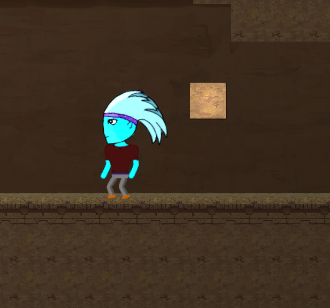
\includegraphics[width=6cm]{images/tyrek/the_lore_puzzle_lvl1.png}
	\caption{Miejsce rozpoczęcia puzzli. Przykład z projektu The Lore}
\end{figure}

W momencie naciśnięcia przycisku akcji kamera zbliża się do obiektu, czyli podświetlonej płytki. Następnie widzimy animację otwierającej się płytki sprawiającej wrażenie, iż ścianka jest przesuwana przez gracza.
\begin{figure}[h]
	\centering
	\includegraphics[width=7cm]{images/tyrek/otwieraniePuzzli.png}
	\caption{Animacja rozpoczęcia puzzli. Przykład z projektu The Lore}
\end{figure}

Po skończonej animacji rozpoczynamy mini-grę. Oprócz bloczków z kolejnością, na ekranie widzimy również dwa przyciski i cyfrę zero. Przyklad:
\begin{figure}[h]
	\centering
	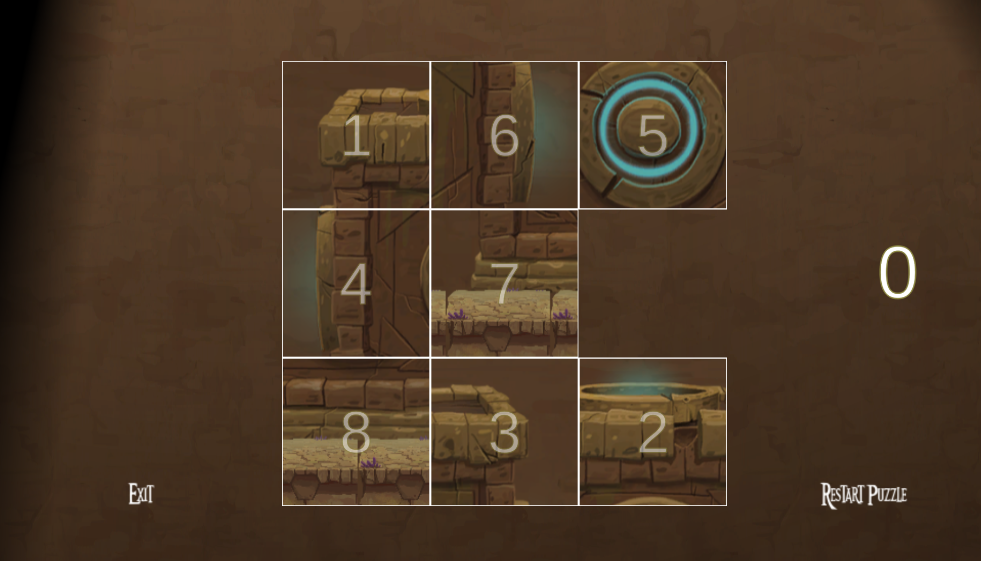
\includegraphics[width=7cm]{images/tyrek/puzzlebuttons.png}
	\caption{Cały interfejs mini-gry puzzle. Przykład z gry The Lore}
\end{figure}
Gdzie \textbf{Exit} kończy rozgrywkę, przenosząc nas z powrotem w miejsce, w którym rozpoczynaliśmy zagadkę, \textbf{Restart Puzzle} powoduje ponowne rozlosowanie puzzli, odwołując się do akcji w klasie \textbf{PuzzleActionsButtons}, czyli tej samej, która uruchamiana jest w przypadku, gdy puzzle nie mają rozwiązania. Dodatkowo po prawej stronie widnieje informacja ile ruchów do tej pory wykonaliśmy rozwiązując zagadkę. Jest to dość istotna informacja dla gracza, gdyż to od ilości ruchów zależy ile punktów doświadczenia zdobędzie za rozwiązanie tej zagadki. Zastosowany wzór dla gry The Lore wygląda następująco:

$$
y = \left\{ \begin{array}{ll}
5 & \textrm{gdy $x>=250$}\\
100 - (x / 25) * 10 & \textrm{gdy $x<250$}\\
\end{array} \right.
$$
Gdzie \textbf{x} jest liczbą wykonanych ruchów.
Po zakończeniu mini-gry jesteśmy informowani o ilości zdobytego doświadczenia. Ponownie widzimy animację przesuwającej się płytki, tym razem zamykającej się.
\begin{figure}[h]
	\centering
	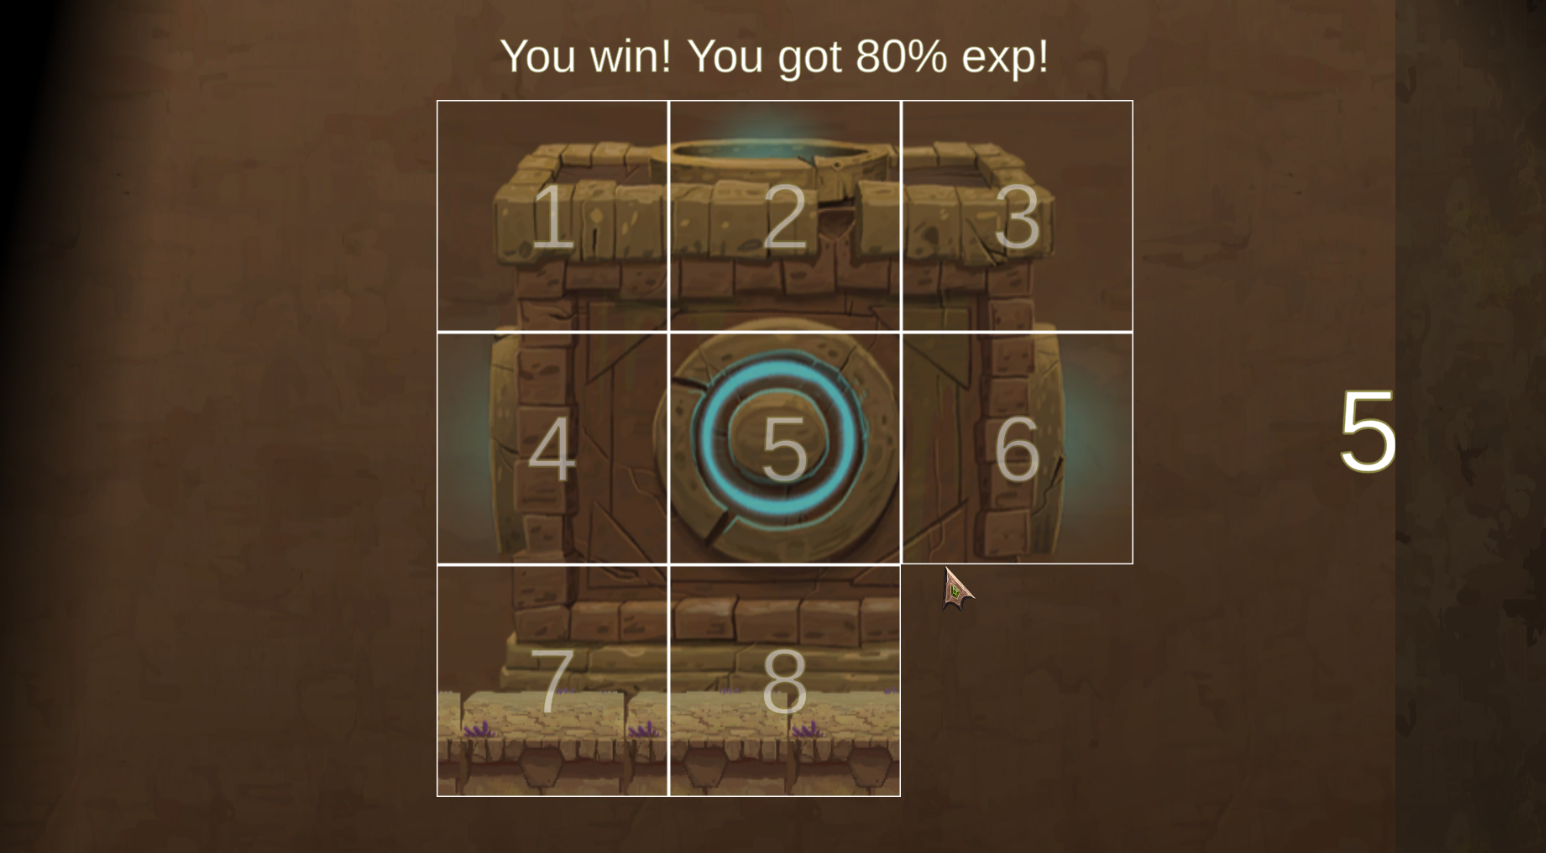
\includegraphics[width=7cm]{images/tyrek/puzzle_end.png}
	\caption{Wygrana rozgrywka puzzle. Przykład z gry The Lore}
\end{figure}

Każdą mini-grę puzzle można wykonać w grze tylko jeden raz. Ponowne próby są niemożliwe, a o tym, iż zagadka została zakończona, jesteśmy informowani przez fakt, iż płytka symbolizująca mini-grę nie jest podświetlona.

\begin{figure}[h]
	\centering
	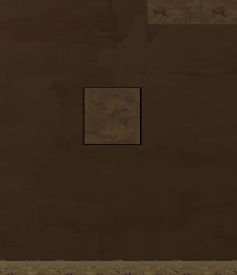
\includegraphics[width=5cm]{images/tyrek/puzzleWin.png}
	\caption{Wygaszona płytka. Przykład z gry The Lore}
\end{figure}

\subsection{Przedstawienie przykładu w innych grach}
Lorem ipsum dolor sit amet, consectetur adipiscing elit. Etiam quis commodo odio, vel pulvinar risus. Quisque ac lacus urna. Aliquam ullamcorper leo non nisl fringilla.

\section{Zagadka z rurami}
\subsection{Omówienie zagadnienia}
\subsection{Algorytmika}
\subsection{Przedstawienie przykładu w grze The Lore}
\subsection{Przedstawienie przykładu w innych grach}

\section{Zagadka z otwieraniem skrzyni}
\subsection{Omówienie zagadnienia}
\subsection{Algorytmika}
\subsection{Przedstawienie przykładu w grze The Lore}
\subsection{Przedstawienie przykładu w innych grach}

\section{Labirynt}
\subsection{Omówienie zagadnienia}
\subsection{Algorytmika}
\subsection{Przedstawienie przykładu w innych grach}

\chapter{Fizyka postaci}
\section{Tworzenie postaci}
\subsection{Omówienie zagadnienia procesu tworzenia postaci}
\subsection{Proces graficzny tworzenia postaci}
\subsection{Wdrożenie postaci do projektu w Unity}
\subsection{Sposoby animowania postaci}

\section{Poruszanie się}
\subsection{Omówienie zagadnienia}
\subsection{Fizyka w grach 2D, a w prawdziwym świecie}
\subsection{Poruszanie się oraz kolizje postaci}
\subsection{Skakanie} 
\subsection{Otoczenie wpływające na fizykę postaci}
\subsection{Umiejętności związane z poruszaniem się}

\begin{thebibliography}{9}
\bibitem{projekt}
Robert K. Wysocki, Rudd McGary: Efektywne zarz¹dzanieprojektami. Wydanie III, ISBN: 83-7361-861-9, dostęp w internecie 26.01.2020r.
http://pdf.onepress.pl/efzapr/efzapr-1.pdf

\bibitem{zagadka_logiczna} 
Wikipedia, Wolna Encyklopedia.” Wikimedia Foundation, Inc. July 17, 2002, dostęp 07.01.2020r.
https://pl.wikipedia.org/wiki/Zagadka

\bibitem{rebus} 
Wikipedia, Wolna Encyklopedia.” Wikimedia Foundation, Inc. July 17, 2002, dostęp 07.01.2020r.
https://pl.wikipedia.org/wiki/Rebus

\bibitem{przesuwane_puzzle}
Wikipedia, Wolna Encyklopedia.” Wikimedia Foundation, Inc. July 17, 2002, dostęp 07.01.2020r.
https://en.wikipedia.org/wiki/15\_puzzle

\bibitem{puzzle}
Wikipedia, Wolna Encyklopedia.” Wikimedia Foundation, Inc. July 17, 2002, dostęp 07.01.2020r.
https://pl.wikipedia.org/wiki/Puzzle

\bibitem{scena}
Unity Documentation, dostęp 09.01.2020r.
https://docs.unity3d.com/Manual/CreatingScenes.html

\bibitem{gameobject}
Unity Documentation, dostęp 09.01.2020r.
https://docs.unity3d.com/ScriptReference/GameObject.html

\bibitem{solvablePuzzle}
Geeks for geeks. Check instance 8 puzzle solvable, dostęp 26.01.2020r.
https://www.geeksforgeeks.org/check-instance-8-puzzle-solvable/

\end{thebibliography}


\end{document}
